% -*- TeX-PDF-mode: t -*-

\documentclass[usepdftitle=false,hyperref={pdfpagelabels=false},t]{beamer}
\usepackage{beamerthemeshadow}
\usepackage[T1]{fontenc}
\usepackage{lmodern}
\usepackage{tikz}
\usepackage{xspace}
\usepackage{graphicx}

\usepackage{pgfpages}
%\setbeameroption{show notes on second screen=bottom}
%\setbeameroption{show only notes}
%\setbeamerfont{note page}{size=\footnotesize}
\setbeamertemplate{note page}[plain]

%\def\hardframe{1}
\def\hardframe{1-}

\usetikzlibrary{arrows}
\usetikzlibrary{calc}
\usetikzlibrary{shapes.arrows}
\usetikzlibrary{shapes.misc}
\usetikzlibrary{shapes.symbols}

\title{Decentralized~Deduplication in~SAN~Cluster~File~Systems}

\author[]{\hspace{.5em} Austin T. Clements$^*$ \\[1em]
  Irfan Ahmad \and Murali Vilayannur \and Jinyuan Li}
\institute{VMWare, Inc. \qquad $^*$MIT CSAIL}
%\date{July 17, 2009}
\date{}

% http://www.tug.org/mail-archives/pdftex/2007-December/007480.html
% This screws up blending, but at least doesn't throw us into CMYK if
% there is any alpha
\pdfpageattr {/Group << /S /Transparency /I true /CS /DeviceRGB>>}

\setbeamertemplate{navigation symbols}{}

%
% PGF layers and images
%

\pgfdeclarelayer{background}
\pgfdeclarelayer{background1}
\pgfdeclarelayer{foreground}

\pgfdeclareimage[width=1cm]{disk}{figures/disk.pdf}
\pgfdeclareimage[width=1cm]{cpu}{figures/cpu.pdf}
% Derived from CX3-40 data sheet at
% http://www.emc.com/collateral/hardware/data-sheet/c1148-clariion-cx3-ds.pdf
\pgfdeclareimage[width=1cm]{cx3-40}{figures/cx3-40.jpg}
\pgfdeclareimage[width=1cm]{server-vms}{figures/server-vms.pdf}
\pgfdeclareimage[width=1cm]{server-onevm}{figures/server-onevm.pdf}
\pgfdeclareimage[width=1cm]{xpvm}{figures/xpvm.pdf}
%\pgfdeclareimage[height=2cm]{file}{figures/file.pdf}
\pgfdeclareimage[width=1cm]{onevm}{figures/onevm.pdf}
\pgfdeclareimage[width=1cm]{pool}{figures/pool.pdf}
\pgfdeclareimage[width=2cm]{server-novm}{figures/server-novm.pdf}

%
% Standard colors
%

\definecolor{unique}{HTML}{3990c4} % Dark blue
\definecolor{shared}{HTML}{8cc63e} % Dark green
\definecolor{index}{HTML}{b3d6eb}  % Light blue
\definecolor{dedup}{HTML}{d7ebba}  % Light green
\definecolor{dedup stroke}{HTML}{898989}

\definecolor{shadeout}{HTML}{3991c4}

%
% TikZ bar styles
%

% Key sample for bar graphs
\tikzset{key box/.style={minimum width=.33cm,minimum height=.33cm,
    inner sep=0pt,label={right:#1}}}

% Bar nodes
\def\vbarfactor{0.005cm}
\tikzset{vbar/.style={anchor=south,minimum width=0.5cm,
    minimum height=#1*\vbarfactor,inner sep=0pt,shading angle=90}}
\tikzset{hbar/.style={anchor=west,minimum height=0.5cm,
    minimum width=#1*\hbarfactor,inner sep=0pt}}

% General bar fill
\tikzset{bar fill/.style={shade=axis,
    top color=white!50!#1,bottom color=black!50!#1,middle color=#1}}

% Space usage bars
\tikzset{unique bar/.style={draw=black,bar fill=unique}}
\tikzset{shared bar/.style={draw=black,bar fill=shared}}
\tikzset{index bar/.style={draw=black,bar fill=index}}
\tikzset{dedup bar/.style={draw=dedup stroke,fill=dedup}}

% Bar graph bars
\tikzset{base bar/.style={unique bar}}
\tikzset{dede bar/.style={shared bar}}

%
% Misc TikZ styles
%

\tikzset{gfx/.style={inner sep=0pt,outer sep=0pt}}

\tikzset{notice circle/.style={line width=.13cm,red,
    postaction={draw=yellow,line width=.1cm}}}

\tikzset{vshadeout/.style={shade=axis,top color=shadeout,bottom color=white}}
\tikzset{lshadeout/.style={shade=axis,right color=shadeout,left color=white}}

\tikzset{indexptr-unique/.style={bar fill=unique}}
\tikzset{indexptr-shared/.style={bar fill=shared}}

\tikzset{disk block/.style={
    minimum width=.6cm,minimum height=.6cm,draw,fill=#1!40!white}}

\tikzset{wlog entry/.style={rounded rectangle,anchor=west,
    minimum width=1.8cm,inner sep=2pt,
    draw=#1!50!black,fill=#1!20!white}}
\tikzset{wlog box/.style={draw=white!61!black,fill=white!93!black}}

\tikzset{show bounds/.style={execute at end picture={
      \draw[dotted] (current bounding box.south west)
      rectangle (current bounding box.north east);
    }}}

\definecolor{dedupcell0}{rgb:hsb}{0,1,1}
\definecolor{dedupcell1}{rgb:hsb}{0.0833333,1,1}
\definecolor{dedupcell2}{rgb:hsb}{0.166667,1,1}
\definecolor{dedupcell3}{rgb:hsb}{0.25,1,1}
\definecolor{dedupcell4}{rgb:hsb}{0.333333,1,1}
\definecolor{dedupcell5}{rgb:hsb}{0.416667,1,1}
\definecolor{dedupcell6}{rgb:hsb}{0.5,1,1}
\definecolor{dedupcell7}{rgb:hsb}{0.583333,1,1}
\definecolor{dedupcell8}{rgb:hsb}{0.666667,1,1}
\definecolor{dedupcell9}{rgb:hsb}{0.75,1,1}
\definecolor{dedupcell10}{rgb:hsb}{0.833333,1,1}
\definecolor{dedupcell11}{rgb:hsb}{0.916667,1,1}
\tikzset{dedupcell-0-0-0/.style={fill=dedupcell8,dedupcell-keep}}
\tikzset{dedupcell-0-0-1/.style={fill=dedupcell11,dedupcell-free}}
\tikzset{dedupcell-0-0-2/.style={fill=dedupcell4,dedupcell-free}}
\tikzset{dedupcell-0-1-0/.style={fill=dedupcell0,dedupcell-keep}}
\tikzset{dedupcell-0-1-1/.style={fill=dedupcell5,dedupcell-free}}
\tikzset{dedupcell-0-1-2/.style={fill=dedupcell6,dedupcell-free}}
\tikzset{dedupcell-0-2-0/.style={fill=dedupcell10,dedupcell-free}}
\tikzset{dedupcell-0-2-1/.style={fill=dedupcell3,dedupcell-free}}
\tikzset{dedupcell-0-2-2/.style={fill=dedupcell2,dedupcell-free}}
\tikzset{dedupcell-0-3-0/.style={fill=dedupcell7,dedupcell-free}}
\tikzset{dedupcell-0-3-1/.style={fill=dedupcell9,dedupcell-keep}}
\tikzset{dedupcell-0-3-2/.style={fill=dedupcell1,dedupcell-free}}
\tikzset{dedupcell-1-0-0/.style={fill=dedupcell4,dedupcell-keep}}
\tikzset{dedupcell-1-0-1/.style={fill=dedupcell10,dedupcell-free}}
\tikzset{dedupcell-1-0-2/.style={fill=dedupcell0,dedupcell-free}}
\tikzset{dedupcell-1-1-0/.style={fill=dedupcell7,dedupcell-free}}
\tikzset{dedupcell-1-1-1/.style={fill=dedupcell9,dedupcell-free}}
\tikzset{dedupcell-1-1-2/.style={fill=dedupcell3,dedupcell-keep}}
\tikzset{dedupcell-1-2-0/.style={fill=dedupcell11,dedupcell-keep}}
\tikzset{dedupcell-1-2-1/.style={fill=dedupcell1,dedupcell-free}}
\tikzset{dedupcell-1-2-2/.style={fill=dedupcell5,dedupcell-keep}}
\tikzset{dedupcell-1-3-0/.style={fill=dedupcell8,dedupcell-free}}
\tikzset{dedupcell-1-3-1/.style={fill=dedupcell2,dedupcell-free}}
\tikzset{dedupcell-1-3-2/.style={fill=dedupcell6,dedupcell-free}}
\tikzset{dedupcell-2-0-0/.style={fill=dedupcell11,dedupcell-free}}
\tikzset{dedupcell-2-0-1/.style={fill=dedupcell2,dedupcell-free}}
\tikzset{dedupcell-2-0-2/.style={fill=dedupcell5,dedupcell-free}}
\tikzset{dedupcell-2-1-0/.style={fill=dedupcell1,dedupcell-free}}
\tikzset{dedupcell-2-1-1/.style={fill=dedupcell3,dedupcell-free}}
\tikzset{dedupcell-2-1-2/.style={fill=dedupcell8,dedupcell-free}}
\tikzset{dedupcell-2-2-0/.style={fill=dedupcell10,dedupcell-free}}
\tikzset{dedupcell-2-2-1/.style={fill=dedupcell4,dedupcell-free}}
\tikzset{dedupcell-2-2-2/.style={fill=dedupcell7,dedupcell-free}}
\tikzset{dedupcell-2-3-0/.style={fill=dedupcell0,dedupcell-free}}
\tikzset{dedupcell-2-3-1/.style={fill=dedupcell9,dedupcell-free}}
\tikzset{dedupcell-2-3-2/.style={fill=dedupcell6,dedupcell-keep}}
\tikzset{dedupcell-3-0-0/.style={fill=dedupcell6,dedupcell-free}}
\tikzset{dedupcell-3-0-1/.style={fill=dedupcell5,dedupcell-free}}
\tikzset{dedupcell-3-0-2/.style={fill=dedupcell0,dedupcell-free}}
\tikzset{dedupcell-3-1-0/.style={fill=dedupcell9,dedupcell-free}}
\tikzset{dedupcell-3-1-1/.style={fill=dedupcell10,dedupcell-keep}}
\tikzset{dedupcell-3-1-2/.style={fill=dedupcell2,dedupcell-keep}}
\tikzset{dedupcell-3-2-0/.style={fill=dedupcell7,dedupcell-keep}}
\tikzset{dedupcell-3-2-1/.style={fill=dedupcell3,dedupcell-free}}
\tikzset{dedupcell-3-2-2/.style={fill=dedupcell4,dedupcell-free}}
\tikzset{dedupcell-3-3-0/.style={fill=dedupcell11,dedupcell-free}}
\tikzset{dedupcell-3-3-1/.style={fill=dedupcell1,dedupcell-keep}}
\tikzset{dedupcell-3-3-2/.style={fill=dedupcell8,dedupcell-free}}
\definecolor{tswlog11}{rgb:hsb}{0.109612,1,1}
\definecolor{tswlog12}{rgb:hsb}{0.10674,1,1}
\definecolor{tswlog13}{rgb:hsb}{0.794793,1,1}
\def\tswloga#1{\ifcase #1\relax\or
f4bea9..\or f2a4d2..\or 0e7a26..
\fi}
\definecolor{tswlog21}{rgb:hsb}{0.804705,1,1}
\definecolor{tswlog22}{rgb:hsb}{0.0674246,1,1}
\definecolor{tswlog23}{rgb:hsb}{0.0325895,1,1}
\def\tswlogb#1{\ifcase #1\relax\or
15ba2b..\or d5e341..\or bc6887..
\fi}
\definecolor{tswlog31}{rgb:hsb}{0.00940564,1,1}
\definecolor{tswlog32}{rgb:hsb}{0.882848,1,1}
\definecolor{tswlog33}{rgb:hsb}{0.98708,1,1}
\def\tswlogc#1{\ifcase #1\relax\or
ab7373..\or 4ee207..\or 9b1f28..
\fi}
\definecolor{tswlog41}{rgb:hsb}{0.987381,1,1}
\definecolor{tswlog42}{rgb:hsb}{0.978421,1,1}
\definecolor{tswlog43}{rgb:hsb}{0.830434,1,1}
\def\tswlogd#1{\ifcase #1\relax\or
9b575b..\or 94c9c9..\or 288bc7..
\fi}
\def\tswlog#1{\ifcase #1\relax\or
\expandafter\tswloga\or \expandafter\tswlogb\or \expandafter\tswlogc\or \expandafter\tswlogd
\fi}
\definecolor{index0}{rgb:hsb}{0.794793,1,1}
\tikzset{indexptr-0/.style={indexptr-shared}}
\definecolor{index1}{rgb:hsb}{0.804705,1,1}
\tikzset{indexptr-1/.style={indexptr-shared}}
\definecolor{index2}{rgb:hsb}{0.923789,1,1}
\tikzset{indexptr-2/.style={indexptr-unique}}
\definecolor{index3}{rgb:hsb}{0.00940564,1,1}
\tikzset{indexptr-3/.style={indexptr-unique}}
\definecolor{index4}{rgb:hsb}{0.0325895,1,1}
\tikzset{indexptr-4/.style={indexptr-unique}}
\definecolor{index5}{rgb:hsb}{0.0408744,1,1}
\tikzset{indexptr-5/.style={indexptr-shared}}
\definecolor{index6}{rgb:hsb}{0.0674246,1,1}
\tikzset{indexptr-6/.style={indexptr-unique}}
\definecolor{index7}{rgb:hsb}{0.10674,1,1}
\tikzset{indexptr-7/.style={indexptr-shared}}
\definecolor{index8}{rgb:hsb}{0.109612,1,1}
\tikzset{indexptr-8/.style={indexptr-unique}}
\def\indexhash#1{\ifcase #1
0e7a26..\or 15ba2b..\or 6cd412..\or ab7373..\or bc6887..\or c277d6..\or d5e341..\or f2a4d2..\or f4bea9..
\fi}
\def\wloghash#1{\ifcase #1
6cd412..\or 12067c..\or c277d6..
\fi}
\definecolor{wlog0}{rgb:hsb}{0.923789,1,1}
\definecolor{wlog1}{rgb:hsb}{0.799644,1,1}
\definecolor{wlog2}{rgb:hsb}{0.0408744,1,1}

\def\bindvmfs#1{
  \path (#1.north west)
    +(39.3144pt,-26.7371pt) coordinate (#1-vm-1)
    +(76.2361pt,-48.4621pt) coordinate (#1-vm-2)
    +(158.216pt,-26.7371pt) coordinate (#1-vm-3)
    +(195.137pt,-48.4621pt) coordinate (#1-vm-4)
    +(104.541pt,-195.969pt) coordinate (#1-disk)
    +(72.1408pt,-195.969pt) coordinate (#1-diskside)
    +(104.541pt,-183.569pt) coordinate (#1-disktop)
  ;
}
\def\bindflow#1{
  \path (#1.north west)
    +(64.8916pt,-88.0194pt) coordinate (#1-vm-2)
    +(123.589pt,-67.2664pt) coordinate (#1-wlog-1)
    +(123.589pt,-87.1709pt) coordinate (#1-wlog-2)
    +(64.8916pt,-117.013pt) coordinate (#1-vm-3)
    +(64.8916pt,-136.917pt) coordinate (#1-vm-4)
    +(123.589pt,-116.164pt) coordinate (#1-wlog-3)
    +(123.589pt,-136.069pt) coordinate (#1-wlog-4)
    +(64.8916pt,-68.115pt) coordinate (#1-vm-1)
    +(174.156pt,-102.513pt) coordinate (#1-idx)
    +(239.271pt,-67.2664pt) coordinate (#1-mreq-1)
    +(239.271pt,-87.1709pt) coordinate (#1-mreq-2)
    +(239.271pt,-116.164pt) coordinate (#1-mreq-3)
    +(239.271pt,-136.069pt) coordinate (#1-mreq-4)
  ;
}
\def\flowwmontowloga#1{
  ($(#1.north west)+(98.1015pt,-42.0993pt)$)
  -- ($(#1.north west)+(98.1015pt,-90.3445pt)$)
  -- ($(#1.north west)+(106.701pt,-90.3445pt)$)
  -- ($(#1.north west)+(106.701pt,-91.9927pt)$)
  -- ($(#1.north west)+(113.126pt,-88.1697pt)$)
  -- ($(#1.north west)+(106.701pt,-84.3696pt)$)
  -- ($(#1.north west)+(106.701pt,-85.995pt)$)
  -- ($(#1.north west)+(102.826pt,-85.995pt)$)
  -- ($(#1.north west)+(102.826pt,-70.4968pt)$)
  -- ($(#1.north west)+(106.701pt,-70.4968pt)$)
  -- ($(#1.north west)+(106.701pt,-72.1451pt)$)
  -- ($(#1.north west)+(113.126pt,-68.3221pt)$)
  -- ($(#1.north west)+(106.701pt,-64.5219pt)$)
  -- ($(#1.north west)+(106.701pt,-66.1473pt)$)
  -- ($(#1.north west)+(102.826pt,-66.1473pt)$)
  -- ($(#1.north west)+(102.826pt,-42.0993pt)$)
  -- ($(#1.north west)+(98.1015pt,-42.0993pt)$)
  -- cycle
}
\def\flowwlogtoldupa#1{
  ($(#1.north west)+(141.975pt,-43.789pt)$)
  -- ($(#1.north west)+(137.825pt,-49.6952pt)$)
  -- ($(#1.north west)+(139.625pt,-49.6952pt)$)
  -- ($(#1.north west)+(139.625pt,-66.3607pt)$)
  -- ($(#1.north west)+(131.139pt,-66.3607pt)$)
  -- ($(#1.north west)+(131.139pt,-70.7102pt)$)
  -- ($(#1.north west)+(139.625pt,-70.7102pt)$)
  -- ($(#1.north west)+(139.625pt,-85.9908pt)$)
  -- ($(#1.north west)+(131.139pt,-85.9908pt)$)
  -- ($(#1.north west)+(131.139pt,-90.3403pt)$)
  -- ($(#1.north west)+(144.35pt,-90.3403pt)$)
  -- ($(#1.north west)+(144.35pt,-49.6952pt)$)
  -- ($(#1.north west)+(146.15pt,-49.6952pt)$)
  -- ($(#1.north west)+(141.975pt,-43.789pt)$)
  -- cycle
}
\def\flowidxtoldupa#1{
  ($(#1.north west)+(152.025pt,-43.789pt)$)
  -- ($(#1.north west)+(156.175pt,-49.6952pt)$)
  -- ($(#1.north west)+(154.375pt,-49.6952pt)$)
  -- ($(#1.north west)+(154.375pt,-85.9908pt)$)
  -- ($(#1.north west)+(167.104pt,-85.9908pt)$)
  -- ($(#1.north west)+(167.104pt,-90.3403pt)$)
  -- ($(#1.north west)+(149.65pt,-90.3403pt)$)
  -- ($(#1.north west)+(149.65pt,-49.6952pt)$)
  -- ($(#1.north west)+(147.85pt,-49.6952pt)$)
  -- ($(#1.north west)+(152.025pt,-43.789pt)$)
  -- cycle
}
\def\flowlduptoidxa#1{
  ($(#1.north west)+(199.55pt,-40.4022pt)$)
  -- ($(#1.north west)+(199.55pt,-90.3445pt)$)
  -- ($(#1.north west)+(190.95pt,-90.3445pt)$)
  -- ($(#1.north west)+(190.95pt,-91.9927pt)$)
  -- ($(#1.north west)+(184.525pt,-88.1697pt)$)
  -- ($(#1.north west)+(190.95pt,-84.3696pt)$)
  -- ($(#1.north west)+(190.95pt,-85.995pt)$)
  -- ($(#1.north west)+(194.825pt,-85.995pt)$)
  -- ($(#1.north west)+(194.825pt,-40.4022pt)$)
  -- ($(#1.north west)+(199.55pt,-40.4022pt)$)
  -- cycle
}
\def\flowlduptomreqa#1{
  ($(#1.north west)+(203.725pt,-41.8164pt)$)
  -- ($(#1.north west)+(203.725pt,-90.3445pt)$)
  -- ($(#1.north west)+(214.267pt,-139.295pt)$)
  -- ($(#1.north west)+(221.942pt,-139.295pt)$)
  -- ($(#1.north west)+(221.942pt,-140.943pt)$)
  -- ($(#1.north west)+(228.367pt,-137.12pt)$)
  -- ($(#1.north west)+(221.942pt,-133.32pt)$)
  -- ($(#1.north west)+(221.942pt,-134.945pt)$)
  -- ($(#1.north west)+(218.067pt,-134.945pt)$)
  -- ($(#1.north west)+(214.667pt,-119.447pt)$)
  -- ($(#1.north west)+(221.942pt,-119.447pt)$)
  -- ($(#1.north west)+(221.942pt,-121.095pt)$)
  -- ($(#1.north west)+(228.367pt,-117.272pt)$)
  -- ($(#1.north west)+(221.942pt,-113.472pt)$)
  -- ($(#1.north west)+(221.942pt,-115.098pt)$)
  -- ($(#1.north west)+(213.867pt,-115.098pt)$)
  -- ($(#1.north west)+(208.45pt,-89.2947pt)$)
  -- ($(#1.north west)+(208.45pt,-41.8164pt)$)
  -- ($(#1.north west)+(203.725pt,-41.8164pt)$)
  -- cycle
}
\def\flowmreqtoxdupa#1{
  ($(#1.north west)+(260.769pt,-43.789pt)$)
  -- ($(#1.north west)+(256.619pt,-49.6952pt)$)
  -- ($(#1.north west)+(258.419pt,-49.6952pt)$)
  -- ($(#1.north west)+(258.419pt,-66.3607pt)$)
  -- ($(#1.north west)+(246.821pt,-66.3607pt)$)
  -- ($(#1.north west)+(246.821pt,-70.7102pt)$)
  -- ($(#1.north west)+(258.419pt,-70.7102pt)$)
  -- ($(#1.north west)+(258.419pt,-85.9908pt)$)
  -- ($(#1.north west)+(246.821pt,-85.9908pt)$)
  -- ($(#1.north west)+(246.821pt,-90.3403pt)$)
  -- ($(#1.north west)+(263.144pt,-90.3403pt)$)
  -- ($(#1.north west)+(263.144pt,-65.9715pt)$)
  -- ($(#1.north west)+(263.144pt,-49.6952pt)$)
  -- ($(#1.north west)+(264.944pt,-49.6952pt)$)
  -- ($(#1.north west)+(260.769pt,-43.789pt)$)
  -- cycle
}
\def\flowwmontowlogb#1{
  ($(#1.north west)+(98.1015pt,-163.469pt)$)
  -- ($(#1.north west)+(98.1015pt,-114.658pt)$)
  -- ($(#1.north west)+(106.701pt,-114.658pt)$)
  -- ($(#1.north west)+(106.701pt,-113.01pt)$)
  -- ($(#1.north west)+(113.126pt,-116.833pt)$)
  -- ($(#1.north west)+(106.701pt,-120.633pt)$)
  -- ($(#1.north west)+(106.701pt,-119.008pt)$)
  -- ($(#1.north west)+(102.826pt,-119.008pt)$)
  -- ($(#1.north west)+(102.826pt,-134.506pt)$)
  -- ($(#1.north west)+(106.701pt,-134.506pt)$)
  -- ($(#1.north west)+(106.701pt,-132.858pt)$)
  -- ($(#1.north west)+(113.126pt,-136.681pt)$)
  -- ($(#1.north west)+(106.701pt,-140.481pt)$)
  -- ($(#1.north west)+(106.701pt,-138.856pt)$)
  -- ($(#1.north west)+(102.826pt,-138.856pt)$)
  -- ($(#1.north west)+(102.826pt,-163.469pt)$)
  -- ($(#1.north west)+(98.1015pt,-163.469pt)$)
  -- cycle
}
\def\flowwlogtoldupb#1{
  ($(#1.north west)+(141.975pt,-161.214pt)$)
  -- ($(#1.north west)+(137.825pt,-155.308pt)$)
  -- ($(#1.north west)+(139.625pt,-155.308pt)$)
  -- ($(#1.north west)+(139.625pt,-138.642pt)$)
  -- ($(#1.north west)+(130.573pt,-138.642pt)$)
  -- ($(#1.north west)+(130.573pt,-134.293pt)$)
  -- ($(#1.north west)+(139.625pt,-134.293pt)$)
  -- ($(#1.north west)+(139.625pt,-119.012pt)$)
  -- ($(#1.north west)+(130.573pt,-119.012pt)$)
  -- ($(#1.north west)+(130.573pt,-114.663pt)$)
  -- ($(#1.north west)+(144.35pt,-114.663pt)$)
  -- ($(#1.north west)+(144.35pt,-155.308pt)$)
  -- ($(#1.north west)+(146.15pt,-155.308pt)$)
  -- ($(#1.north west)+(141.975pt,-161.214pt)$)
  -- cycle
}
\def\flowidxtoldupb#1{
  ($(#1.north west)+(152.025pt,-161.214pt)$)
  -- ($(#1.north west)+(156.175pt,-155.308pt)$)
  -- ($(#1.north west)+(154.375pt,-155.308pt)$)
  -- ($(#1.north west)+(154.375pt,-119.012pt)$)
  -- ($(#1.north west)+(167.104pt,-119.012pt)$)
  -- ($(#1.north west)+(167.104pt,-114.663pt)$)
  -- ($(#1.north west)+(149.65pt,-114.663pt)$)
  -- ($(#1.north west)+(149.65pt,-155.308pt)$)
  -- ($(#1.north west)+(147.85pt,-155.308pt)$)
  -- ($(#1.north west)+(152.025pt,-161.214pt)$)
  -- cycle
}
\def\flowlduptoidxb#1{
  ($(#1.north west)+(199.55pt,-166.015pt)$)
  -- ($(#1.north west)+(199.55pt,-114.658pt)$)
  -- ($(#1.north west)+(190.95pt,-114.658pt)$)
  -- ($(#1.north west)+(190.95pt,-113.01pt)$)
  -- ($(#1.north west)+(184.525pt,-116.833pt)$)
  -- ($(#1.north west)+(190.95pt,-120.633pt)$)
  -- ($(#1.north west)+(190.95pt,-119.008pt)$)
  -- ($(#1.north west)+(194.825pt,-119.008pt)$)
  -- ($(#1.north west)+(194.825pt,-166.015pt)$)
  -- ($(#1.north west)+(199.55pt,-166.015pt)$)
  -- cycle
}
\def\flowlduptomreqb#1{
  ($(#1.north west)+(203.725pt,-164.884pt)$)
  -- ($(#1.north west)+(203.725pt,-114.658pt)$)
  -- ($(#1.north west)+(214.267pt,-65.7083pt)$)
  -- ($(#1.north west)+(221.942pt,-65.7083pt)$)
  -- ($(#1.north west)+(221.942pt,-64.06pt)$)
  -- ($(#1.north west)+(228.367pt,-67.883pt)$)
  -- ($(#1.north west)+(221.942pt,-71.6831pt)$)
  -- ($(#1.north west)+(221.942pt,-70.0578pt)$)
  -- ($(#1.north west)+(218.067pt,-70.0578pt)$)
  -- ($(#1.north west)+(214.667pt,-85.5559pt)$)
  -- ($(#1.north west)+(221.942pt,-85.5559pt)$)
  -- ($(#1.north west)+(221.942pt,-83.9077pt)$)
  -- ($(#1.north west)+(228.367pt,-87.7307pt)$)
  -- ($(#1.north west)+(221.942pt,-91.5308pt)$)
  -- ($(#1.north west)+(221.942pt,-89.9055pt)$)
  -- ($(#1.north west)+(213.867pt,-89.9055pt)$)
  -- ($(#1.north west)+(208.45pt,-115.708pt)$)
  -- ($(#1.north west)+(208.45pt,-164.884pt)$)
  -- ($(#1.north west)+(203.725pt,-164.884pt)$)
  -- cycle
}
\def\flowmreqtoxdupb#1{
  ($(#1.north west)+(260.769pt,-161.214pt)$)
  -- ($(#1.north west)+(256.619pt,-155.308pt)$)
  -- ($(#1.north west)+(258.419pt,-155.308pt)$)
  -- ($(#1.north west)+(258.419pt,-138.642pt)$)
  -- ($(#1.north west)+(247.104pt,-138.642pt)$)
  -- ($(#1.north west)+(247.104pt,-134.293pt)$)
  -- ($(#1.north west)+(258.419pt,-134.293pt)$)
  -- ($(#1.north west)+(258.419pt,-119.012pt)$)
  -- ($(#1.north west)+(247.104pt,-119.012pt)$)
  -- ($(#1.north west)+(247.104pt,-114.663pt)$)
  -- ($(#1.north west)+(263.144pt,-114.663pt)$)
  -- ($(#1.north west)+(263.144pt,-139.031pt)$)
  -- ($(#1.north west)+(263.144pt,-155.308pt)$)
  -- ($(#1.north west)+(264.944pt,-155.308pt)$)
  -- ($(#1.north west)+(260.769pt,-161.214pt)$)
  -- cycle
}
\def\bindlayers#1{
  \path (#1.north west)
    +(73.8075pt,-140.579pt) coordinate (#1-diskleft)
  ;
}


%
% Standard pictures and drawing definitions
%

\newcommand\myrightarrow{\tikz \node[draw=red,fill=yellow,
  shape=single arrow,minimum height=1cm,scale=0.33] {};
  % This puts in the right amount of space
  {}}

\tikzset{
  cell-0-0/.style={opacity=.7,fill=white},
  cell-0-1/.style={opacity=.7,fill=white},
  cell-1-0/.style={opacity=.7,fill=white},
  cell-1-1/.style={opacity=.7,fill=white}
}
\newcommand{\vmdk}[3][]{
  \xvmdk[#1]{#2}{#3}{onevm}
}
\newcommand{\xvmdk}[4][]{
  \node[inner sep=1pt,#1] (#2) {\pgfuseimage{#4}};
  \only<#3>{
    \begin{scope}[yslant=-.58,x=.55cm,y=.55cm,xshift=-3pt,yshift=-3pt]
      \foreach \x in {0,1} {
        \foreach \y in {0,1} {
          \fill[cell-\x-\y]
               (\x,-\y) rectangle +(-1,1)
               +(-.5,.5) node[minimum width=.55cm] (#2-\x-\y) {};
        }
      }
      \draw
        \foreach \y in {1,0,-1} {(-1,\y) -- (1,\y)}
        \foreach \x in {1,0,-1} {(\x,-1) -- (\x,1)};
    \end{scope}
  }
}

\tikzset{
  block arrow/.style={->,line width=2pt},
  cow arrow/.style={->,line width=2pt,dotted}
}
\makeatletter
\tikzset{
  di/idxptr os/.store in=\di@idxptr@os,
  di/idx shift by/.store in=\di@idx@shift@by,
  di/disk os/.store in=\di@disk@os,
  di/avmdk os/.store in=\di@avmdk@os,
  di/avmdk grid os/.store in=\di@avmdk@grid@os,
  di/avmdk cells os/.store in=\di@avmdk@cells@os,
  di/bvmdk os/.store in=\di@bvmdk@os,
  di/bvmdk b1 os/.store in=\di@bvmdk@bone@os,
  di/bvmdk b2 os/.store in=\di@bvmdk@btwo@os,
  di/pool os/.store in=\di@pool@os,
  di/pool b1 os/.store in=\di@pool@bone@os,
  di/pool b2 os/.store in=\di@pool@btwo@os,
}
\def\di@idxptr@os{1-}
\def\di@idx@shift@by{0}
\def\di@disk@os{1-}
\def\di@avmdk@os{0}
\def\di@avmdk@grid@os{0}
\def\di@avmdk@cells@os{0}
\def\di@bvmdk@os{0}
\def\di@bvmdk@bone@os{0}
\def\di@bvmdk@btwo@os{0}
\def\di@pool@os{1-}
\def\di@pool@bone@os{0}
\def\di@pool@btwo@os{0}
\tikzset{index entry/.style={fill=#1!20!white,
    minimum width=1.8cm,minimum height=.55cm}}
\tikzset{index ptr/.style={indexptr-#1,
    minimum height=.55cm,minimum width=.4cm}}
\tikzset{disk-index8/.style={},disk-index5/.style={},
  disk-wlog0/.style={},disk-index2/.style={},
  disk-wlog2/.style={}}
\newcommand{\drawindex}[1][]{
  \begin{scope}[#1]
    \node[overlay] (idx-top) {};
    \def\p{(idx-top.south)}
    \foreach \i in {0,...,8} {
      \node[index entry=index\i,below,outer sep=0pt] (idx-\i)
        at \p {\indexhash{\i}};
      \node<\di@idxptr@os>[index ptr=\i,right] (idxptr-\i)
        at (idx-\i.east) {};
      \ifnum \i=0\relax
        \gdef\p{($(idx-0.south)+\di@idx@shift@by*(0,-.55cm)$)}
      \else
        \xdef\p{(idx-\i.south)}
      \fi
    }
    \draw (idx-0.north west) rectangle (idx-8.south east);
    \draw<\di@idxptr@os>
      (idxptr-0.north west) rectangle (idxptr-8.south east);

    \only<\di@disk@os>{
      \node[inner sep=0pt,scale=2] (disk) at (8.4,-4) {\pgfuseimage{disk}};
      \foreach \a/\s in {18/index8,90/wlog2,162/wlog0,234/index2,306/index5} {
        \path (disk.north) +(\a:1cm and .4cm)
          node[above,disk block=\s,disk-\s] (disk-\s) {};
      }
    }

    \begin{scope}[xshift=4.6cm,yshift=-1.55cm]
      \only<\di@avmdk@cells@os>{
        \tikzset{
          cell-0-0/.style={fill=wlog1,opacity=.4},
          cell-1-0/.style={fill=wlog0,opacity=.4},
          cell-0-1/.style={fill=wlog2,opacity=.4},
          cell-1-1/.style={fill=index8,opacity=.4},
        }
      }
      \only<\di@avmdk@os>{\vmdk{avmdk}{\di@avmdk@grid@os}}
    \end{scope}

    \begin{scope}[xshift=4.6cm,yshift=-3.05cm]
      \only<\di@bvmdk@bone@os>{\tikzset{cell-0-0/.style={fill=index2,opacity=.4}}}
      \only<\di@bvmdk@btwo@os>{\tikzset{cell-1-0/.style={fill=index5,opacity=.4}}}
      \only<\di@bvmdk@os>{\vmdk{bvmdk}{1-}}
    \end{scope}

    \path<\di@pool@os>[overlay] (4.6cm,-4.6cm)
              node[scale=2,inner sep=0pt] {\pgfuseimage{pool}}
              +(-.4cm,.15cm) coordinate (pool-1)
              +(.4cm,0cm) coordinate (pool-2);
    \node<\di@pool@bone@os>[disk block=index5] (pb1) at (pool-1) {};
    \node<\di@pool@btwo@os>[disk block=wlog0] (pb2) at (pool-2) {};
  \end{scope}
}
\makeatother

\newcommand\mlnode[1]{\begin{tabular}{c}#1\end{tabular}}

\makeatletter
\newenvironment{steps}{%
  \bgroup
  \def\steps@indent{}%
  \def\steps@arrow{}%
  \newcommand<>{\step}[1]{%
    \onslide##2{\steps@indent\steps@arrow ##1}%
    \xdef\steps@indent{\quad\steps@indent}%
    \gdef\steps@arrow{\myrightarrow} \\%
  }%
  \begin{tabular}{l}%
}{%
  \end{tabular}%
  \egroup
}
\makeatother


\begin{document}

\frame{\titlepage}

\iffalse

\newcommand{\xpvm}{
  node[scale=2,anchor=north west,inner sep=0pt] {\pgfuseimage{xpvm}}
}
\tikzset{xpgridxform/.style=
  {yslant=-.58,x=.55cm,y=.7cm,xshift=-.26cm,yshift=-.1cm}}
\newcommand{\xpgrid}{
  {[xpgridxform]
    \foreach \y in {0,...,-3} {(0,\y) -- (4,\y)}
    \foreach \x in {0,...,4} {(\x,0) -- (\x,-3)}
  }
}
\newcommand{\xpblocks}[1]{
  \begin{scope}[xpgridxform]
    \foreach \x in {0,...,3} {
      \foreach \y in {0,...,2} {
        \fill[dedupcell-#1-\x-\y]
             (\x,-\y) rectangle +(1,-1)
             +(0.5,-0.5) node (dedupcell-#1-\x-\y) {};
      }
    }
  \end{scope}
}

\begin{frame}{Deduplication}
  % Virtualized data centers waste tons of expensive disk space storing
  % duplicate data.  If you've got 100 XP VM's, you're storing 99 too
  % many copies of XP.

  % (Anim) Horizontal, then vertical lines.  Fade colors in, or add
  % tiles one at a time.  Add all circles, or add one at a time.
  % Slide red blocks together.  Fade away other blocks.

  % XXX COW
  \begin{tikzpicture}
    \foreach \n in {0,...,3} {
      \begin{scope}[xshift=\n*2.8cm]
        \path (0,0) \xpvm;
        \tikzset{dedupcell-keep/.style={opacity=.4}}
        \only<-4>{
          \tikzset{dedupcell-free/.style={dedupcell-keep}}
        }
        \only<5->{
          \tikzset{dedupcell-free/.style={fill=white}}
        }
        \only<3->{\xpblocks{\n}}
        \onslide<2->{\draw (0,0) \xpgrid;}
        \only<4>{
          \foreach \nn in {dedupcell-0-1-0,dedupcell-1-0-2,
            dedupcell-2-3-0,dedupcell-3-0-2} {
            \draw[notice circle]
              (\nn.center) circle (.5);
          }
        }
      \end{scope}
    }
  \end{tikzpicture}

  \vspace{1em}
  \begin{center}
    \begin{steps}
      \step<2->{Divide VM disks into 4~KB blocks}
      \step<3->{Compute block hashes}
      \step<4->{Index and detect identical hashes}
      \step<5->{Replace with COW references}
    \end{steps}
  \end{center}
\end{frame}

\begin{frame}{Deduplication in Virtual Infrastructures}
  \begin{itemize}
  \item<+-> Live, primary storage.  Not archival.
  \item<+-> Must minimize IO overhead.
  \item<+-> The shared file system is decentralized, so DeDe must be,
    too.
  \end{itemize}
\end{frame}

\newcommand{\dedebox}[2]{
  \path[draw=unique,
  shade,top color=index!50!white,bottom color=index,
  rounded corners]
  (0,0) rectangle +(4,-7.8);
}

\begin{frame}{DeDe}
  % Origin is the current baseline with the standard 1cm margin.  Page
  % width is 128mm.
  % \begin{tikzpicture}[overlay,xshift=-1cm,yshift=1em]
  %   \begin{scope}[xshift=2mm]
  %     \dedebox{}{}
  %   \end{scope}
  %   \begin{scope}[xshift=44mm]
  %     \dedebox{}{}
  %   \end{scope}
  %   \begin{scope}[xshift=86mm]
  %     \dedebox{}{}
  %   \end{scope}
  % \end{tikzpicture}

  % XXX 2x3 evenly spaced grid with icons to left of each point

  \onslide<+>{}

  {\bf Decentralized} \\ \onslide<+->{Cooperatively
    performs block-level deduplication of the shared file system while
    retaining all direct-access performance advantages of SAN's.  The
    shared disk itself is the only centralized component.}
  \vspace{1em}

  {\bf Efficient} \\ \onslide<+->{Minimizes IO impact by detecting
    duplicates as a background process and by keeping unique blocks
    mutable and sequential.}
  \vspace{2em}

  {\bf Layered} \\ \onslide<+->{Builds atop an existing SAN file
    system with minor interface additions.  Takes advantage of
    existing locking, disk layout, and file system abstractions.}
  \vspace{1em}
\end{frame}

\fi


\begin{frame}<\hardframe>{Storage Area Networks}
  % XXX Can we say internal VMware VDI deployment?
  \note{Storage area networks form the backbone of most virtualized
    data centers.  They provide block-level SCSI access to shared
    disks to multiple hosts simultaneously.  This direct access
    enables high-performance shared file systems such as VMware's
    VMFS, which, in turn, lets us run lots and lots of virtual
    machines off the shared file system.  However, now that we're
    running lots and lots of VM's, we have a problem: lots and lots of
    duplicate data.  This is especially bad if we're running a virtual
    desktop infrastructure, or VDI, where we have, say, hundreds of XP
    desktop VM's running from our data center.  In fact, to see just
    how much of a problem this was, we took 113 VM's from a live,
    corporate VDI cluster, or 1.3~TB worth of actual disk data and
    deduplicated it.  We were left with 237~GB.  That's a 5x
    reduction.  Clearly this is a problem.}

  \begin{center}
    \begin{tikzpicture}
      \node<1->[gfx] (vmfs) {\includegraphics{overlays/vmfs-base.pdf}};
      \bindvmfs{vmfs}
      \node<2->[gfx] {\includegraphics{overlays/vmfs-scsi.pdf}};
      \node<3->[gfx] {\includegraphics{overlays/vmfs-platform.pdf}};
      \only<3-> {
        \foreach \vm in {1,...,4} {
          \begin{scope}[overlay,shift=(vmfs-vm-\vm),scale=1.2]
            \def\img{onevm}
            \only<4->{\def\img{xpvm}}
            \xvmdk[scale=1.2]{vm-\vm}{0}{\img}
          \end{scope}
        }
      }
      \begin{scope}[overlay]
        \coordinate (bar left) at (-4.75cm,0 |- vmfs-disk);
        \onslide<5-> {
          \def\hbarfactor{0.0068cm}
          \def\st{unique bar}
          \only<6->{\def\st{dedup bar}}
          \node[\st,hbar=1300] (fullbar) at (bar left) {};
          \node[above] at (fullbar.north east) {1.3~TB};
        }
        \only<6-> {
          \path (bar left)
          node[unique bar,hbar=237] (shared) {} ++(237*\hbarfactor,0)
          node[hbar=1063] (dedupbar) {};
          \node[above] at (shared.north east) {237~GB};
        }
        \only<7-> {
          \node<+->[shape=starburst,fill=yellow,draw=red,font={\bf}]
          at (dedupbar) {5X reduction};
        }
      \end{scope}
    \end{tikzpicture}
  \end{center}

  % Show two hosts with arrows pointing to a shared disk.  Label arrows
  % as SCSI.  Show four generic VM's running on the hosts.  Show XP
  % running on the four VM's.  Show 1.3~TB bar below disk.  Show 237~GB
  % bar with ``5x reduction'' in starburst.
\end{frame}

\begin{frame}<\hardframe>{Deduplication}
  \note{We can eliminate this duplication using content hashes to
    identify and share duplicate data.  For example, imagine
    that each time a host updates a block, it computes the hash of
    that block's new contents and looks it up in an index stored on
    the shared disk.  If there's already a block with that hash, it
    simply reuses that block.  Otherwise, it writes it to some unused
    space on disk and adds it to the index.

    Now, this works great if you've got a central host with exclusive
    control over the file system, but it doesn't work at all in our
    decentralized setting for a couple of reasons.}

  \begin{center}
    \pgfsetlayers{background,main}
    \begin{tikzpicture}
      \node<1->[gfx] (vmfs) {\includegraphics{overlays/vmfs-base.pdf}};
      \bindvmfs{vmfs}
      %\node<1->[gfx] {\includegraphics{overlays/vmfs-scsi.pdf}};
      \node<1->[gfx] {\includegraphics{overlays/vmfs-platform.pdf}};
      \begin{scope}[overlay]
        \foreach \vm in {1,...,4} {
          \begin{scope}[shift=(vmfs-vm-\vm),scale=1.2]
            \ifnum 1=\vm
            \only<4->{
              \tikzset{cell-0-0/.style={fill=index5,opacity=.4}}
            }
            % \only<7->{
            %   \tikzset{cell-1-1/.style={fill=index5,opacity=.4}}
            % }
            \fi
            \xvmdk[scale=1.2]{vm-\vm}{2-}{xpvm}
          \end{scope}
        }
        \draw<3->[notice circle] (vm-1-0-0) circle (.5);
        \node<5->[gfx,anchor=south,scale=.7] (idx) at (vmfs.south -| -5cm,0) {
          \begin{tikzpicture}
            %\tikzset{index entry/.append style={text opacity=.4}}
            \tikzset{indexptr-unique/.style={indexptr-shared}}
            \drawindex[di/disk os=0,di/pool os=0,di/idxptr os=0]
            %\node<6->[right] at (idxptr-5.east) {Checkmark};
            \draw<6>[notice circle,overlay,
              transform canvas={scale around={1.4:(idx-5)}}]
              (idx-5) ellipse (0.9 and 0.3);
            %\draw[notice circle] (idx-5) circle (.5);
          \end{tikzpicture}
        };
        \begin{pgfonlayer}{background}
          \path<5->[lshadeout] (vmfs-diskside) -- (idx.south east) --
          (idx.north east) -- cycle;
        \end{pgfonlayer}
        \tikzset{disk-none/.style={draw=none,fill=none}}
        \colorlet{none}{white}
        \only<7->{
          \foreach \a/\s in {18/none,90/index5,162/none,234/none,306/none} {
            \path (vmfs-disktop) +(\a:1cm and .4cm)
              node[above,disk block=\s,disk-\s] (disk-\s) {};
          }
          \draw[block arrow] (vm-1-0-0.center) to[out=0,in=90] (disk-index5);
          %\draw[block arrow] (idxptr-5.center) to (disk-index5);
          %\draw[notice circle] (vm-1-1-1) circle (.5);
        }
        \only<8-> {
          \draw[block arrow] (disk-index5) -- (idx.east |- disk-index5);
        }
      \end{scope}
    \end{tikzpicture}
  \end{center}

  % (Naive approach.)  Same base diagram as previous slide.
  % Overlay block grids on VM's and put some blocks over the disk.
  % Circle some VM block.  Color that block.  Show the index next to the
  % disk with a shade-out.  Put a checkmark next to the right entry.
  % Draw an arrow from the entry to the existing disk block.  Circle and
  % color another block.  Put an X next to the index.  Add a block above
  % the disk and draw an arrow from the VM block to the disk block.  Add
  % entry to the index and draw an arrow from the entry to the new disk
  % block.
\end{frame}

\begin{frame}[c]{The Problem}
  \onslide<1->{{\bf Slow} --- Lots of IO in the write path.  Can't cache
    the index.}
  \vspace{1em}
  \note<1>{First of all, it's slow.  VM IO used to translate pretty
    directly into actual disk IO.  Now we have to perform random IO to
    a complicated on-disk structure every time we write a block.  Most
    systems solve this problem using aggressive index caching, but we
    can't do that in our multi-host setting.}

  \onslide<2->{{\bf Very Slow} --- Writes require allocation and thus
    coordination. \\
    \qquad No hope of disk locality.
  }
  \vspace{1em}
  \note<2>{Actually, it's very slow.  Write require allocation and
    thus coordination between hosts.  Oh, and forget any hope of
    retaining disk locality.}

  \onslide<3->{{\bf Hopelessly Slow} --- Multi-host lock contention on
    shared index.}
  \note<3>{But, really, it's just hopelessly slow.  Every single write
    requires access to a shared structure.  Not only does this result
    in lock contention, but any locking at all is extremely expensive
    in this environment.}

  % XXX Hmm.  It's only once you optimize for unique blocks that the
  % need to modify metadata on other hosts comes up.
  %\only<4->{{\bf Impossible} --- 
\end{frame}

\def\nflow#1{\node[inner sep=0pt,outer sep=0pt] {\includegraphics{overlays/flow-#1.pdf}};}

\begin{frame}{Three-Stage Deduplication}
  % XXX Live file system (not archival), out-of-band dedup
  \begin{center}
    \unskip
    \only<1>{\large \textcolor{red}{De}centralized
      \textcolor{red}{De}duplication}
    \note<1>{To address these problems, we designed and implemented a
      decentralized deduplication engine for SAN cluster file
      systems.}
    \only<2->{\large DeDe}
    \note<2>{DeDe for short.}
    \begin{tikzpicture}
      \onslide<3->{\node[gfx] {\includegraphics{overlays/stages-base.pdf}};}
    \end{tikzpicture}
  \end{center}
  \note<3>{DeDe divides the deduplication process into three separate
    stages: write monitoring, local deduplication, and cross-host
    deduplication.}
  \begin{itemize}
  \item<4-> Process duplicates efficiently, in large batches
  \item<4-> Minimize contention on the index
  \item<4-> Unique blocks remain mutable and sequential
  \end{itemize}
  \note<4>{This approach lets us run the deduplication stages only
    periodically, which means we can process duplicates efficiently
    and in large batches.  Because we're processing things in large
    batches, this in turn lets us minimize contention on the shared
    index.  Furthermore, because this approach lets us partition
    metadata changes, we'll be able to keep unique blocks mutable and
    sequential.}
\end{frame}

\begin{frame}<3->{Three-Stage Deduplication}
  % Write monitoring is happening independently without coordination
  % Don't touch the index in cross-host deduplication
  % Review at end.  Only time there's any coordination in the
  % merge-requests.
  \begin{center}
    \unskip
    \only<2->{\large DeDe}
    \pgfsetlayers{background,background1,main,foreground}
    \begin{tikzpicture}
      \tikzset{flow arrow/.style={draw=black,fill=yellow,line width=0.5pt}}
      \tikzset{light flow arrow/.style={draw=black!30!white,fill=yellow!30!white,line width=0.5pt}}
      \node[gfx] (flow) {\includegraphics{overlays/flow-base.pdf}};
      \bindflow{flow}
      \only<3-5> {\nflow{wmona} \nflow{ldupa} \nflow{xdupa}}
      \note<3>{These three stages form a pipeline...}
      \begin{pgfonlayer}{background}
        \only<4-> {\nflow{hosts}}
        \only<4-5> {\nflow{wmonb} \nflow{ldupb} \nflow{xdupb}}
        \note<4>{Which every host in the cluster executes
          independently.}
        \only<5-> {\nflow{disk}}
        \note<5>{The stages communicate with each both on each
          host and between hosts using regular files stored in the
          shared file system.}
      \end{pgfonlayer}
      \begin{pgfonlayer}{foreground}
        \only<6-> {\nflow{gray}}
        \only<6-7> {\nflow{wmona} \nflow{wmonb}}
        \only<6> {\nflow{host2vm}}
      \end{pgfonlayer}
      \only<6-> {
        \foreach \n in {1,...,4} {
          \begin{scope}[shift={(flow-vm-\n)},scale=.5]
            \vmdk[scale=.5]{vm-\n}{1-}
          \end{scope}
        }
      }
      \note<6>{In the first stage, write monitoring, each host
        continuously monitors its own writes to the file system.}
      \only<7-> {
        {
          \only<8->{\tikzset{flow arrow/.style={light flow arrow}}}
          \path[flow arrow]
          \flowwmontowloga{flow}
          \flowwmontowlogb{flow};
        }
        \begin{pgfonlayer}{foreground}
          \foreach \vm/\os in {1/-10,2/-10,3/-13,4/-13} {
            \node[scale=.4] at (flow-wlog-\vm) {
              \begin{tikzpicture}
                \node (wlog) {};
                \path[wlog box,use as bounding box]
                  (wlog.west) ++(-0.1cm,-.15cm) rectangle +(1.85cm,-1.7cm);
                \foreach \e in {1,...,3} {
                  \path<\os> (wlog.west) +(0,-.5cm)
                  node[wlog entry=tswlog\vm\e,text opacity=.4] (wlog)
                  {\tswlog{\vm}{\e}};
                }
              \end{tikzpicture}
            };
          }
        \end{pgfonlayer}
        \nflow{wlogs}
      }
      \note<7>{Each host periodically records the hashes of all
        recently modified blocks in on-disk, per-file write logs.}
      \only<8-12> {
        \begin{pgfonlayer}{foreground}
          \nflow{ldupa}
        \end{pgfonlayer}
      }
      \note<8>{Once a host has accumulated large enough write logs, it
        executes the local deduplication phase.  This phase consumes
        the write logs produced by the write monitor...}
      \only<9-12> {
        \begin{pgfonlayer}{background}
          \nflow{idxlocka}
        \end{pgfonlayer}
      }
      \only<9-> {
        \node[scale=.4] at (flow-idx) {
          \begin{tikzpicture}
            \tikzset{index entry/.append style={text opacity=.4}}
            \drawindex[di/disk os=0,di/pool os=0]
            \draw<12>[notice circle,overlay,
              transform canvas={scale around={2.5:(idx-1.center)}}]
              (idx-1.center) ellipse (0.7 and 0.3);
          \end{tikzpicture}
        };
        \nflow{idx}
      }
      \note<9>{This locks a shared index of block hashes, again stored
        in the shared file system.}
      \only<10-> {
        \begin{pgfonlayer}{background1}
          \only<13->{\tikzset{flow arrow/.style={light flow arrow}}}
          \path[flow arrow] \flowidxtoldupa{flow};
          \path[flow arrow] \flowwlogtoldupa{flow};
        \end{pgfonlayer}
      }
      \note<10>{And performs a batch merge of the information on
        recently modified blocks from the host's write logs...}
      \only<11-> {
        {
          \only<13->{\tikzset{flow arrow/.style={light flow arrow}}}
          \path[flow arrow] \flowlduptoidxa{flow};
        }
      }
      \note<11>{... into the index.}
      \draw<12>[notice circle] (vm-1-0-0.center) circle (0.4);
      \note<12>{During this process, if it discovers that any new
        block hashes match blocks already in the index, it can
        deduplicate those blocks.}
      \only<13> {
        \begin{pgfonlayer}{foreground}
          \nflow{ldupb}
        \end{pgfonlayer}
        \begin{pgfonlayer}{background}
          \nflow{idxlockb}
        \end{pgfonlayer}
      }
      \only<13-> {
        \begin{pgfonlayer}{background1}
          \only<14->{\tikzset{flow arrow/.style={light flow arrow}}}
          \path[flow arrow]
          \flowwlogtoldupb{flow}
          \flowidxtoldupb{flow}
          \flowlduptoidxb{flow};
        \end{pgfonlayer}
      }
      \note<13>{And the other host goes through a similar process at
        some other time.}
      \note<14>{Of course, there's a catch.}
      \only<15>{
        \begin{pgfonlayer}{foreground}
          \nflow{ldupa}
        \end{pgfonlayer}
        \draw[notice circle] (vm-1-1-0) circle (0.4);
        \draw[notice circle] (vm-4-0-0) circle (0.4);
      }
      \note<15>{The first time we find a duplicate block, the indexed
        block may be in a file locked by a different host.  Because
        we're in a decentralized setting, we can't just go clobbering
        the other file's block pointers.  We need to coordinate.}
      \only<16>{
        \begin{pgfonlayer}{foreground}
          \nflow{ldupa} \nflow{ldupb}
        \end{pgfonlayer}
      }
      \only<16->{
        {
          \only<17->{\tikzset{flow arrow/.style={light flow arrow}}}
          \path[flow arrow] \flowlduptomreqa{flow};
          \path[flow arrow] \flowlduptomreqb{flow};
        }
        % XXX Locking
        \foreach \vm in {1,...,4} {
          \node[scale=.4] at (flow-mreq-\vm) {
            \begin{tikzpicture}
              % XXX Should use different block colors
              \path[wlog box,use as bounding box]
                (-0.925cm,1cm) rectangle +(1.85cm,-1.7cm);
              \node[font=\Huge] at (90:.6cm) (top) {?};
              \node[disk block=index0] at (210:.6cm) {};
              \node[disk block=index8] at (330:.6cm) {};
            \end{tikzpicture}
          };
        }
        \nflow{mreq}
      }
      \note<16>{When this happens, the local deduplication stage
        % XXX Check what we call these in the paper
        produces on-disk, per-file merge requests.}
      \only<17>{
        \begin{pgfonlayer}{foreground}
          \nflow{xdupa} \nflow{xdupb}
        \end{pgfonlayer}
        % XXX Locking
      }
      \only<17->{
        \begin{pgfonlayer}{background1}
          \path[flow arrow] \flowmreqtoxdupa{flow};
          \path[flow arrow] \flowmreqtoxdupb{flow};
        \end{pgfonlayer}
      }
      \note<17>{In the final stage, hosts periodically check for merge
        requests for the files they have open.  If they find one, they
        verify that the request is still valid and rewrite the local
        file's block pointers accordingly.}
    \end{tikzpicture}
  \end{center}

  % XXX What this gets us
  % Three-stage deduplication allows us to
  %   minimize contention on shared structures and cross-host
  %   communication, perform in-place writes to unique blocks, and
  %   isolate meta-data XXX.}

  % \note<3>{
  %   % Show second host
  %   Each host executes these stages independently and simultaneously,
  %   though the last two stages, which together update the hash index
  %   and eliminate duplicate blocks occur only periodically.
  %   % Show disk
  %   All communication between stages and between hosts is done via
  %   files stored in the shared file system.
  % }

%   \note<4>{
%     % Fade out other stages
%     In the first stage, each host continuously monitors all of its own
%     writes to the file system.
%     % Show write logs
%     It computes the hash of each block that it modifies and
%     periodically records these hashes in on-disk, per-file write logs.
%   }

%   \note<5>{
%     % Fade out other stages, showing just local for host A
%     The next stage happens whenever a host has accumulated large
%     enough write logs.
%     % Show index, locked by host A
%     In this stage, the host locks a shared index and consumes the
%     write logs of all of the files it has open.
%     % Hide write log entries from host A, show updating index arrow
%     It updates the index to reflect recently modified blocks, in the
%     process detecting recently introduced duplicates and eliminating
%     duplicates from files it has open.
%   }

%   \note<6>{
%     % XXX Circle some duplicates as we go along?
%     In the process, the host may discover newly duplicated blocks in
%     files other hosts have open.
%     % Show merge requests for host B, locked by host A
%     It can only modify meta-data of files it has open, so it records
%     such deduplication opportunities in per-file merge requests.
%   }

%   % XXX Want to show cross-over

%   \note<7>{
%     % Fade out other stages, showing just cross for host B.  Host B
%     % merge requests locked by host B.
%     Then, in the third stage, hosts periodically consume and process
%     merge requests for all of the files they have open, completing the
%     deduplication process.

%     % Change index lock to host B
% %    At some other time, the other host will lock the index and update
% %    it to reflect recent modification to the files that host has open.
%   }
\end{frame}

\begin{frame}[c]{Implementation}
  \note<1>{We implemented DeDe atop the VMware ESX hypervisor and
    VMware's VMFS file system.  The implementation consists of a few
    small but important changes to VMFS, a write monitor kernel
    module, an on-disk index structure, and a deduplication daemon.}
  \begin{center}
    \begin{tikzpicture}
      \only<+->{
        \node[gfx] (layers) {\includegraphics{overlays/layers-esx.pdf}};
        \bindlayers{layers}
      }
      \node<+->[gfx] {\includegraphics{overlays/layers-vmfs.pdf}};
      \node<+->[gfx] {\includegraphics{overlays/layers-wmon.pdf}};
      \node<+->[gfx] {\includegraphics{overlays/layers-disk.pdf}};
      \only<.->{
        \node[overlay,below,scale=.5] (idx) at (-2.75cm,-.25cm) {
          \begin{tikzpicture}
            \tikzset{index entry/.append style={text opacity=.4}}
            \drawindex[di/disk os=0,di/pool os=0,di/idxptr os=0]
          \end{tikzpicture}
        };
        % WTF?  My layers-diskleft node doesn't work.
        \path[overlay,lshadeout] (-10mm,-15mm) -- (idx.north east) --
        (idx.south east) -- cycle;
      }
      \node<+->[gfx] {\includegraphics{overlays/layers-dedupd.pdf}};
    \end{tikzpicture}
  \end{center}
\end{frame}

\begin{frame}{VMFS}
  % In addition to the copy-on-write support already in VMFS, we added
  % a new compare-and-share operation.
  \note<1>{The most important change we made to VMFS was to add
    support for a ``compare-and-share'' operation.}
  \begin{center}
    \unskip
    Compare-and-share

    \vspace{1em}
    \begin{tikzpicture}
      \begin{scope}[shift={(-2cm,2cm)}]
        \tikzset{cell-1-0/.style={fill=index0,opacity=.4}}
        \vmdk{a}{1-}
      \end{scope}
      \begin{scope}[shift={(2cm,2cm)}]
        \tikzset{cell-0-0/.style={fill=index0,opacity=.4}}
        \vmdk{b}{1-}
      \end{scope}
      \node[gfx,scale=2] (disk) at (0,0) {\pgfuseimage{disk}};
      \def\blocks{45/index0,135/index0}
      \only<3->{
        \def\blocks{135/index0}
      }
      \foreach \a/\s in \blocks {
        \path (disk.north) ++(0,-.3cm) +(\a:1cm and .4cm)
          node[above,disk block=\s] (disk-\a) {};
      }
      \draw<1-2>[block arrow] (a-1-0.center) to[out=0,in=90] (disk-135);
      \draw<1-2>[block arrow] (b-0-0.center) to[out=180,in=90] (disk-45);
      \draw<2>[block arrow,<->] (disk-135) -- (disk-45)
      node[midway,above,font={\LARGE}] {?};
      \draw<3->[cow arrow] (a-1-0.center) to[out=0,in=90] (disk-135);
      \draw<3->[cow arrow] (b-0-0.center) to[out=180,in=90] (disk-135);
    \end{tikzpicture}

    \vspace{1em}
    \only<4->{DeDe finds duplicates.  VMFS eliminates them.}
  \end{center}
\end{frame}

% \begin{frame}{File System}
%   \begin{center}
%     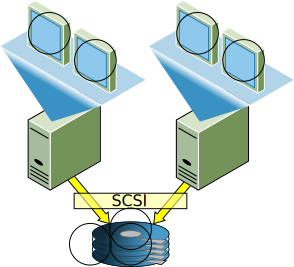
\includegraphics[scale=.4]{../usenix09/figures/vmfs.pdf}
%   \end{center}
%   \begin{itemize}
%   \item<+-> Build atop VMFS, mostly unmodified
%   \item<+-> DeDe obeys file-level locking
%   \item<+-> DeDe never manipulates block addresses directly
%   \item<+-> Two important new interfaces
%     \begin{itemize}
%     \item<+-> Mixed block sizes
%     \item<+-> \emph{Compare-and-share}
%     \end{itemize}
%   \end{itemize}
%   % XXX VMFS already supports block-level copy-on-write
% \end{frame}

\begin{frame}{Write Monitor}
  % Buffering point is too much of a stretch.  Try to say that the
  % index can be stale and we're still correct.
  \begin{center}
    \unskip
    \begin{tikzpicture}[inner sep=0pt]
      \node<1-> (base) {\includegraphics[scale=.6]{overlays/writemon-base.pdf}};
      \node<2-3> {\includegraphics[scale=.6]{overlays/writemon-todisk.pdf}};
      \fill<2->[white,fill opacity=.8,overlay]
        (base.north west) rectangle (base.east |- 0,-1.35);
      \node<2-3> {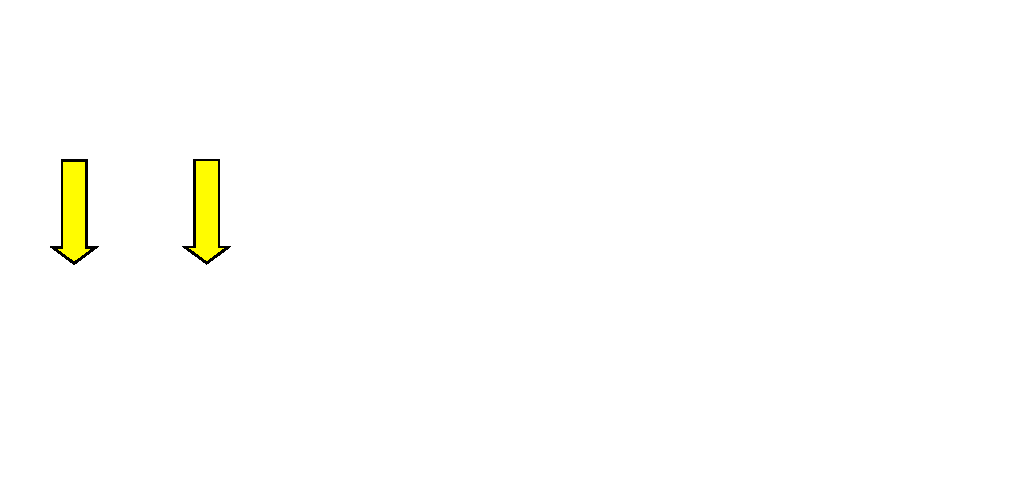
\includegraphics[scale=.6]{overlays/writemon-vmwrites.pdf}};
      \node<2->  {\includegraphics[scale=.6]{overlays/writemon-fs3dedup.pdf}};
      \node<3->  {\includegraphics[scale=.6]{overlays/writemon-log.pdf}};
      \node<4->  {\includegraphics[scale=.6]{overlays/writemon-record.pdf}};
      \node<4->  {\includegraphics[scale=.6]{overlays/writemon-todisk.pdf}};
    \end{tikzpicture}

    \vspace{1em}
    \begin{itemize}
      \item<2-> A lightweight kernel module monitors writes,
        computes hashes
      \item<3-> It buffers the write log in userspace before writing
        it to disk
      \item<5-> Safe to buffer the log because of compare-and-share
      \item<6-> 150~MB of regular writes $\rightarrow$ 1~MB sequential
        log write
    \end{itemize}
  \end{center}
  \note<6>{So, now that we can gather hashes, we need an index so we
    can find them}
\end{frame}

% \begin{frame}{Write Monitor}
%   \begin{center}
%     \unskip
%     \begin{tikzpicture}[inner sep=0pt]
%       \node<1-> (base) {\includegraphics[scale=.6]{overlays/writemon-base.pdf}};
%       \node<2-4> {\includegraphics[scale=.6]{overlays/writemon-todisk.pdf}};
%       \fill<3->[white,fill opacity=.8,overlay]
%         (base.north west) rectangle (base.east |- 0,-1.35);
%       \node<2-4> {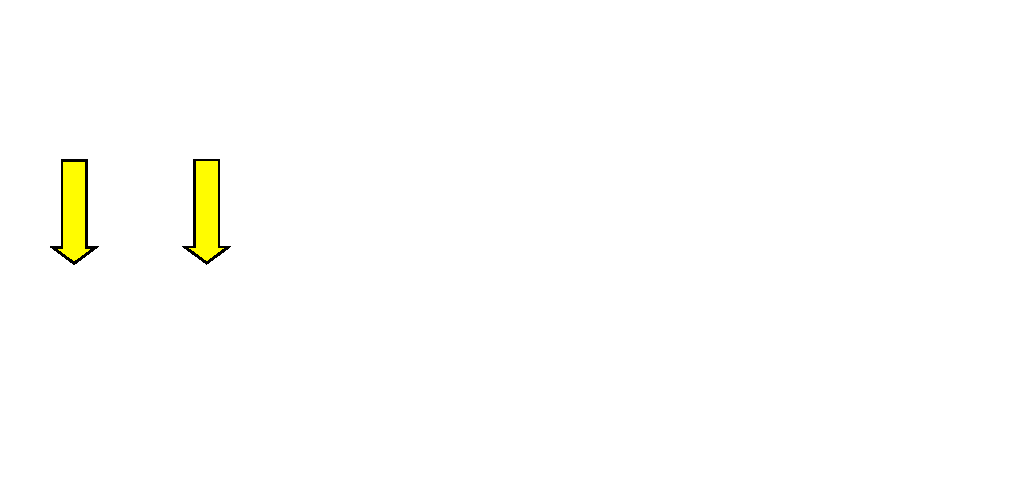
\includegraphics[scale=.6]{overlays/writemon-vmwrites.pdf}};
%       \node<3->  {\includegraphics[scale=.6]{overlays/writemon-fs3dedup.pdf}};
%       \node<4->  {\includegraphics[scale=.6]{overlays/writemon-log.pdf}};
%       \node<5->  {\includegraphics[scale=.6]{overlays/writemon-record.pdf}};
%       \node<5->  {\includegraphics[scale=.6]{overlays/writemon-todisk.pdf}};
%     \end{tikzpicture}

%     \vspace{1em}
%     \begin{steps}
%       \step<2->{VM's write to virtual disks through VMFS}
%       \step<3->{A lightweight kernel module monitors all writes}
%       \step<4->{It streams a compact summary to user space}
%       \step<5->{The log of hashes is flushed to disk periodically}
%     \end{steps}
%   \end{center}
% \end{frame}


% XXX Virtual arena pushes text
\begin{frame}<1-2,4->{The Index}
  % Key
  \begin{tikzpicture}
    \drawindex[di/idxptr os=2-, di/disk os=5-,
      di/bvmdk os=3-, di/bvmdk b1 os=4-5, di/bvmdk b2 os=8-,
      di/pool os=7-, di/pool b1 os=8-]
    \draw<4-5>[block arrow] (idxptr-2.center) to[out=0,in=180] (bvmdk-0-0);
    \draw<5>[block arrow] (bvmdk-0-0.center) to[bend left=20] (disk-index2);

    \draw<8->[cow arrow] (pb1.center) to[out=0,in=180] (disk-index5);
    \draw<8->[cow arrow] (bvmdk-1-0.center) to[out=0,in=180] (disk-index5);

    \draw<9->[block arrow] (idxptr-5.center) to[out=0,in=180] (pb1);
  \end{tikzpicture}

  \begin{itemize}
  \item<1-> Map from hashes to block locators, list sorted by hash
  \item<4-> Unique blocks are located in files and remain mutable
  \item<7-> A virtual arena stores COW references to all shared blocks
  \end{itemize}
\end{frame}

\begin{frame}<\hardframe>{Indexing and Duplicate Elimination}
  % Tiny host icon next to VM's

  % The deduplication process itself is interleaved with updating the
  % index.  Each host independently decides when to perform
  % deduplication based on how much data it has written to the file
  % system combined with user-defined policy (such as only
  % deduplicating during off-peak hours).

  % Suppose that this host decides its time to deduplicate.  A host
  % only processes modifications made to files it has locks on because
  % those are the only files it can manipulate the metadata of.  This
  % host is running just one VM, so it has an exclusive lock on that
  % VM's disk file.

  % First, it opens the write log for the VM's disk.  This contains
  % records for all of the blocks that have been modified in that file
  % since it was last deduplicated against the file system.

  % The host sorts all of these records by hash and then begins
  % scanning the sorted index in tandem with the sorted list of write
  % records, merging the two structures and writing out a brand new
  % index.
  \pgfsetlayers{background,main}
  \begin{tikzpicture}
    \only<7->{\tikzset{di/idx shift by=1}}
    \only<15->{
      \tikzset{indexptr-2/.style={indexptr-shared}}
    }
    \only<16->{
      \tikzset{disk-index2/.style={draw=none,fill=none}}
    }
    \only<20->{
      \tikzset{disk-wlog2/.style={draw=none,fill=none}}
    }
    \drawindex[di/avmdk os=2-,di/avmdk grid os=3-,di/avmdk cells os=4-,
      di/bvmdk os=11-,di/bvmdk b1 os=11-16,di/bvmdk b2 os=18-20,
      di/pool os=13-,di/pool b2 os=14-,di/pool b1 os=18-]
    \begin{pgfonlayer}{background}
      \only<2-4>{
        \node[inner sep=0pt,anchor=north] at ($(avmdk.north)+(0,-.3cm)$)
          {\pgfuseimage{server-novm}};
      }
    \end{pgfonlayer}
    \only<4>{
      % Write log
      \begin{pgfonlayer}{background}
        \path[wlog box]
           (1.95cm,-.15cm) -| (7.1cm,-.65cm)
           -| ($(avmdk.south east)+(0,-.25cm)$)
           -- ($(avmdk.south west)+(-.2cm,.5cm)$)
           |- (1.95cm,-.65cm) -- cycle;
      \end{pgfonlayer}
      \gdef\wlogapos{(3.7cm,-.4cm)}
      \gdef\wlogbpos{(2cm,-.4cm)}
      \gdef\wlogcpos{(5.4cm,-.4cm)}
    }
    \def\afterwlog{}
    \only<5->{
      \gdef\wlogbpos{(wlog1.west) +(0,-.5cm)}
      \gdef\wlogcpos{(wlog0.west) +(0,-.5cm)}
    }
    \only<5>{
      % Sorted write log at top
      \gdef\wlogapos{(1.6cm,-.4cm)}
    }

    % Absent->shared
    \only<6>{
      % wlog1 lined up
      \gdef\wlogapos{(1.6cm,-.4cm |- idxptr-0.south)}
    }
    \only<7->{
      % wlog1 lined up more
      \gdef\wlogapos{(1.6cm,-.4cm |- idxptr-0.south) +(0,-.275cm)}
    }
    \only<6-7>{
      \gdef\afterwlog{
        \draw[->,line width=2pt] (wlog1.west) -- (wlog1.west -| idxptr-0.east);
      }
    }
    \only<8->{
      \begin{pgfonlayer}{background}
        \node[index entry=wlog1,below] (idx-wlog1)
          at (idx-0.south) {\wloghash{1}};
        \only<9->{
          \node[index ptr=unique,right] (idxptr-wlog1)
            at (idx-wlog1.east) {};
        }
      \end{pgfonlayer}
      \only<9>{
        \draw[block arrow]
          (idxptr-wlog1.center) to[out=0,in=180] (avmdk-0-0);
      }
    }
    \only<8-9>{
      % wlog1 lined up more, but invisible (XXX Not working)
      \xdef\wlogbpos{\wlogapos +(0,-.8cm)}
    }

    % Unique->Shared
    \only<10>{
      \gdef\wlogbpos{(1.6cm,-.4cm |- idxptr-2.east)}
      \gdef\afterwlog{
        \draw[->,line width=2pt] (wlog0.west) -- (idxptr-2.east);
      }
    }
    \only<11-16>{
      \gdef\wlogcpos{(1.6cm,-.4cm |- idxptr-2.east) +(0,-.5cm)}
    }
    \only<11-14>{
      \draw[block arrow] (idxptr-2.center) to[out=0,in=180] (bvmdk-0-0);
    }
    \only<15-16>{
      \draw[block arrow] (idxptr-2.center) to[out=0,in=180] (pb2);
    }
    \only<12-13>{
      \draw[block arrow] (avmdk-1-0.center) to[bend left=20] (disk-wlog0);
    }
    \only<12-15>{
      \draw[block arrow] (bvmdk-0-0.center) to[bend left=20] (disk-index2);
    }
    \only<16>{
      \draw[cow arrow]
        (bvmdk-0-0.center) to[bend left=20] (disk-wlog0.north west);
    }
    \only<12>{
      \draw[notice circle] (avmdk-1-0) circle (.5);
      \draw[notice circle] (bvmdk-0-0) circle (.5);
    }
    \only<14-16>{
      \draw[cow arrow] (avmdk-1-0.center) to[bend left=20] (disk-wlog0);
      \draw[cow arrow] (pb2.center) to[out=0] (disk-wlog0);
    }

    % Shared->Shared
    \only<17>{
      \gdef\wlogcpos{(1.6cm,-.4cm |- idxptr-5.east)}
      \gdef\afterwlog{
        \draw[->,line width=2pt] (wlog2.west) -- (idxptr-5.east);
      }
    }
    \only<18-20>{
      \draw[block arrow] (idxptr-5.center) to[out=0,in=180] (pb1);
    }
    \only<19-20>{
      \draw[cow arrow] (pb1.center) to[out=0,in=180] (disk-index5);
      \draw[cow arrow] (bvmdk-1-0.center) to[out=0,in=180] (disk-index5);
    }
    \only<19>{
      \draw[block arrow] (avmdk-0-1.center) to[out=0,in=180] (disk-wlog2);
      \draw[notice circle] (avmdk-0-1) circle (.5);
      \draw[notice circle] (bvmdk-1-0) circle (.5);
    }
    \only<20>{
      \draw[cow arrow] (avmdk-0-1.center) to[out=0,in=180] (disk-index5);
    }
    \only<21>{
      \draw[notice circle] (disk) +(0,.5cm) circle (2);
    }

    \only<4-7>{
      \path \wlogapos node[wlog entry=wlog1] (wlog1) {\wloghash{1}};
    }
    \only<4-10>{
      \path \wlogbpos node[wlog entry=wlog0] (wlog0) {\wloghash{0}};
    }
    \only<4-17>{
      \path \wlogcpos node[wlog entry=wlog2] (wlog2) {\wloghash{2}};
      \afterwlog
    }
  \end{tikzpicture}
\end{frame}

%
% Evaluation
%

\begin{frame}[c]
  \begin{center}
    Whew.
  \end{center}
\end{frame}

\begin{frame}{Evaluation}
  % Space further apart
  \begin{center}
    \onslide<+->{}
    \onslide<+->{How much space does DeDe save?} \\
    \onslide<+->{How much overhead does DeDe introduce?} \\
    \onslide<+->{How fast can DeDe deduplicate?}
  \end{center}
\end{frame}

\begin{frame}{Space Savings: VDI Cluster}
  % Zero thing

  % In order to show that deduplication was actually worth the effort,
  % we analyzed virtual disks from a real, live corporate virtual
  % desktop infrastructure cluster.  (XXX Explain VDI if necessary)
  % These were all Windows XP desktop VM's that have been in active
  % use by non-technical users for six to twelve months.  They were
  % all originally cloned from a small number of base disk images.

  % We analyzed disks from 113 randomly selected VM's, totaling 1.3
  % terabytes of data, not including blocks consisting exclusively of
  % NULL's.

  % (XXX 1.9TB including NULL blocks)

  \note<1>{Of course, I already kind of spoiled the punchline, but
    just in case you missed it, we reduced that 1.3~TB to 237~GB.  Now
    we can look at what that 237~GB consists of.  Only 61~GB of that
    consists of shared blocks.  That means all of that space saving
    comes from repetitions of those 61~GB's of blocks.  Actually, some
    of those blocks are repeated 200,000 times in the original disks.
    That's 800~MB for a single 4~KB block.

    Dede also introduces space overhead.  We have to store an index of
    all of these blocks, not to mention the virtual arena's metadata.}

  \begin{columns}[T]
    \begin{column}{5.5cm}
      \begin{itemize}
      \item Corporate Virtual Desktop Infrastructure cluster
      \item Desktop XP VM's
        %for non-technical departments
      %\item One VM per user
      \item 6--12 months of active use
      \item Originally cloned from small number of base images
      \end{itemize}
    \end{column}
    \begin{column}{4.8cm}
      \begin{tikzpicture}
        \node[inner sep=0pt,scale=1.75,above] (servers) at (0,0)
          {\pgfuseimage{server-vms}\;\;\pgfuseimage{server-vms}};
        \node at (servers) {...};
        \node[inner sep=0pt,scale=1.75,below] at (-.15,-.25) (disk)
          {\pgfuseimage{disk}};
        \onslide<2-> {
          \node[left,inner sep=0pt,rotate=270] (vmbar) at (servers.north)
            {$\left\{\vbox to 2cm {}\right.$};
          \node[above] at (vmbar.west) {113~VM's};
          \node[left,inner sep=0pt] (diskbar) at (disk.west)
            {$\left\{\vbox to .75cm {}\right.$};
          \node[left] at (diskbar.west) {1.3~TB};
       }
      \end{tikzpicture}
    \end{column}
  \end{columns}
\end{frame}

\def\afterbar#1{
  {[x=\hbarfactor]
    node[index bar,hbar=3]    (#1-idxbar)    {} ++(3,0)
    node[unique bar,hbar=173] (#1-uniquebar) {} ++(173,0)
    node[shared bar,hbar=61]  (#1-sharedbar) {} ++(61,0)
  }
}

\begin{frame}[t]{Space Savings: VDI Cluster}
  % 82% reduction at 4K block size
  % 1.3TB -> 235GB (61.1GB in shared blocks)
  % The worst blocks are repeated over 100,000 times.  Each of these
  % blocks alone represents 400 megs of space savings.

  % (/ 6555889 256.0 1024.0) => 25~GB repeated 2x
  % 4~KB repeated 199,927 times => 781~MB
  \begin{center}
    \pgfsetlayers{background,main}
    \begin{tikzpicture}
      \def\hbarfactor{0.0068cm}
      \node<+>[unique bar,hbar=1300] (fullbar) at (0,0) {};
      \node<2->[dedup bar,hbar=1300] (fullbar) at (0,0) {};
      \node<.->[above] at (fullbar.north east) {1.3~TB};
      \node<.->[left=0.2cm,inner sep=0] at (fullbar.west) {\pgfuseimage{disk}};

      \path<+-> (0,0) \afterbar{main} node[hbar=1063] (dedupbar) {};
      \node<.->[above] at (dedupbar.north west) {237~GB};

%      \node<+->[shape=starburst,fill=yellow,draw=red,font={\bf}] at (dedupbar) {82\%};

      \let\mainhbarfactor\hbarfactor
      \def\hbarfactor{0.035cm}
      \path<+-> (.5cm,-2cm) \afterbar{zoom};
      \node<.->[below] at (zoom-uniquebar.south) {\mlnode{173~GB \\ unique}};
      \node<.->[below] at (zoom-sharedbar.south) {\mlnode{61~GB \\ shared}};
      \path<.->[vshadeout]
        (fullbar.south west) -- (main-sharedbar.south east) --
        (zoom-sharedbar.north east) -- (zoom-idxbar.north west) -- cycle;

      % XXX Trying to show the 50 -> 25 GB reduction at 2 references,
      % but the scales of the bars are different, so this looks weird
      %
      % \path<+->[draw]
      % {[x=\mainhbarfactor] ($(fullbar.south east) - (50,0)$)}
      % |- (fullbar.north east) -- (fullbar.south east)
      % -- (zoom-sharedbar.north east) -- (zoom-sharedbar.south east) -|
      % ($(zoom-sharedbar.north east) - (25*\hbarfactor,0)$) -- cycle;

      \node<+->[draw=red,fill=yellow,shape=arrow box,
                arrow box arrows={north:.5cm},anchor=north]
      at (zoom-idxbar.south) {2.7~GB};

      \def\hbarfactor{0.003cm}
      \path<+-> (1cm,-4.5cm) {[x=\hbarfactor]
        node[index bar,hbar=1300] (indexfilebar) {} ++(1300,0)
        node[index bar,hbar=194]  (arenabar) {} ++(194,0)
        node[index bar,hbar=1100] (pbbar) {} ++(1100,0)
      };
      \begin{pgfonlayer}{background}
        \path<.->[vshadeout]
          (zoom-idxbar.south west) -- (zoom-idxbar.south east) --
          (pbbar.north east) -- (indexfilebar.north west) -- cycle;
      \end{pgfonlayer}
      \path<.->[below]
        (indexfilebar.south) node {\mlnode{1.3~GB \\ index file}}
        (arenabar.south)     node {\mlnode{194~MB \\ v. arena}}
        (pbbar.south)        node {\mlnode{1.1~GB \\ FS metadata}};
    \end{tikzpicture}
  \end{center}
\end{frame}

% XXX Linked clones?  I think linked clones are more important than
% the effects of block sizes

\begin{frame}{Runtime Effects}
  \note<1>{What about the runtime overhead?  Most of DeDe runs
    out-of-band precisely to avoid runtime overheads, but we still
    have to worry about the write monitor.  On the other hand, there
    are potential gains to be had from improved disk array caching.
    To measure the effects of these, we ran benchmarks inside a VM
    stored on an EMC CLARiiON CX3-40 SAN.}
  \begin{columns}[T]
    \begin{column}{7cm}
      % \begin{itemize}
      % \item<+-> Primarily out-of-band
      % \item<.-> No IO overhead for unique blocks
      % \end{itemize}

      % \onslide<+->{but...}

      % \begin{itemize}
      % \item<.-> CPU overhead for write monitoring
      % \item<+-> IO overhead from COW specialization
      % \item<+-> IO overhead from 4~KB block size
      % \item<+-> IO \emph{improvement} from caching
      % \end{itemize}
      \begin{itemize}
      \item<+-> Write monitoring
      %\item<.-> COW specialization
      \item<.-> Disk array caching
      \end{itemize}
    \end{column}
    \begin{column}{3.4cm}
      \begin{center}
        \vspace{-2.5em}
        \pgfsetlayers{background,main}
        \begin{tikzpicture}
          \node<+->[inner sep=0pt,scale=1.5,above]
          {\pgfuseimage{server-onevm}};
          \begin{pgfonlayer}{background}
            \onslide<+->{
              \node[below,scale=2.5,label={below:\mlnode{EMC CLARiiON \\ CX3-40}},
                inner sep=0pt] at (0,-.3cm) {\pgfuseimage{cx3-40}};
              \node[shape=single arrow,rotate=270,minimum height=1.5cm,scale=0.5,
                draw=black,fill=yellow] {};
            }
          \end{pgfonlayer}
        \end{tikzpicture}
      \end{center}
    \end{column}
  \end{columns}
\end{frame}

\begin{frame}{Runtime Overhead: Write Monitoring}
  Worst-case benchmark: 100\% sequential write IO, No computation

  \only<+>{}
  \begin{center}
    \begin{tikzpicture}
      \onslide<+-> {
        \path (1cm,1cm) node[base bar,key box={Baseline}] {}
              ++(2.5cm,0) node[dede bar,key box={Write Monitor}] {};

        \def\hbarfactor{0.03cm}
        \path (0,0) node[right,inner sep=0pt] {CPU}
              ++(0,-0.6) node[base bar,hbar=33,label={right:33\%}] (cpu-base) {}
              ++(0,-0.6) node[dede bar,hbar=220,label={right:220\%}] (cpu-dede) {};
        \node[inner sep=0pt,left=0.2cm,scale=1.5] at
        ($(cpu-base.west)!.5!(cpu-dede.west)$) {\pgfuseimage{cpu}};
      }

      \def\hbarfactor{2.59cm}
      \onslide<+-> {
        \path (0,-2.5) node[right,inner sep=0pt] {Bandwidth (MB/s)}
              ++(0,-0.6) node[base bar,hbar=1,label={right:233}] (disk-base) {}
              ++(0,-0.6) node[dede bar,hbar=1,label={right:233}] (disk-dede) {};
        \path (4,-2.5) node[right,inner sep=0pt] {Latency (ms)}
              ++(0,-0.6) node[base bar,hbar=1,label={right:8.6}] {}
              ++(0,-0.6) node[dede bar,hbar=1,label={right:8.6}] {};
        \node[inner sep=0pt,left=0.2cm,scale=1.5] at
        ($(disk-base.west)!.5!(disk-dede.west)$) {\pgfuseimage{disk}};
      }
    \end{tikzpicture}
  \end{center}
\end{frame}

\begin{frame}{Runtime Gains: Disk Array Caching}
  \begin{center}
    Reduced storage footprint \myrightarrow Better caching
    \myrightarrow Less IO

    \vspace{2em}

    \only<+>{}
    \pgfimage<+>[width=9cm]{figures/copied-vs-dedup-0.pdf}
    \pgfimage<+>[width=9cm]{figures/copied-vs-dedup-1.pdf}
    \pgfimage<+>[width=9cm]{figures/copied-vs-dedup-2.pdf}
  \end{center}
\end{frame}

\begin{frame}[c]{Out-of-band Deduplication Rate}
  % Can process 9~GB of new shared blocks per hour.  We believe this
  % is reasonable because we don't expect new *shared* blocks to be
  % introduced that quickly and we can process new unique blocks at
  % the full index scan rate.  So, for example, if a VM is running a
  % database, ...
  \begin{center}
    \begin{tabular}{l@{\hspace{3em}}r@{ }r}
      Index scan & \onslide<2->{6.6 & GB/sec} \\
%      4~KB conversion & \onslide<3->{37.5 & MB/sec} \\
      \only<4->{\color{orange}}COW sharing &
      \onslide<3->{\only<4->{\color{orange}}2.6 &
        \only<4->{\color{orange}}MB/sec}
    \end{tabular}

    \vspace{2em}

    \onslide<5->{
      \myrightarrow 9~GB of new \emph{shared} blocks per hour \\
      (And provisioning can be special-cased)
    }
  \end{center}
\end{frame}

\begin{frame}{Related Work}
  \begin{itemize}
  \item Centralized archival
    \begin{itemize}
    \item Venti
    \item Data Domain
    \item Foundation
    \end{itemize}
  \item Centralized primary storage
    \begin{itemize}
    \item NetApp ASIS
    \item Microsoft Single Instance Store
    \end{itemize}
  \item Distributed
    \begin{itemize}
    \item Farsite
    \end{itemize}
  \item SAN with Coordinator
    \begin{itemize}
    \item DDE
    \end{itemize}
  \end{itemize}
\end{frame}

\begin{frame}{Conclusion}
  % Live file systems, out of band, and decentralized.
  \begin{center}
    \begin{tikzpicture}
        \coordinate (bar left) at (0,0);
        \def\hbarfactor{0.0068cm}
        \node[dedup bar,hbar=1300] (fullbar) at (bar left) {};
        \path (bar left)
        node[unique bar,hbar=237] (shared) {} ++(237*\hbarfactor,0);
    \end{tikzpicture}
    Deduplication is effective.
    \vspace{1em}

    \onslide<2->{
      \begin{tikzpicture}
        \node {\includegraphics[scale=.4]{overlays/decentralized-base.pdf}};
      \end{tikzpicture}

      Deduplication is hard.
      \vspace{1em}
    }

    \onslide<3->{
      \begin{tikzpicture}
        \node {\includegraphics[scale=.5]{overlays/stages-cropped-base.pdf}};
      \end{tikzpicture}

      Three-stage deduplication has only modest performance overhead.
      \vspace{1em}
    }

    \onslide<4->{Thank you.}
  \end{center}

  % DeDe performs block-level deduplication of live, shared file systems
  % without any central coordination.

  % DeDe operates out-of-band from writes and optimizes for unique
  % blocks.

  % DeDe builds atop an existing file system with minimal modifications.

  % DeDe can achieve 80\% space reduction with minor performance
  % overhead.
\end{frame}

% \begin{frame}[c]
%   \begin{center}
%     Thank you!
%   \end{center}
%   % XXX URL or something?  Put something up for question time.
% \end{frame}

\begin{frame}[plain]
\end{frame}

\begin{frame}[c]{Block Sizes, Realigned Partitions, and Linked Clones}
  \begin{center}
    % XXX This figure doesn't get rebuilt automatically.
    \includegraphics[width=108mm]{figures/vmware-it-vdi-bar2.pdf}
  \end{center}
\end{frame}

\begin{frame}{Why Not Use Block Pointers?}
  \begin{itemize}
  \item Dangling pointer problems, garbage collection problems
  \item Block migration problems (Defragmenting, upgrading, etc.)
  \item Locking problems
  \end{itemize}
\end{frame}

\end{document}
